%\begin{figure}[h]
	%\centering
	%\missingfigure{Komponentendiagramm}		
	%\caption{Komponentendiagramm - A}
	%\label{fig:komponentendiagramm-a}
%\end{figure}

%\begin{tcolorbox}
%Die strukturelle Übersicht des zu entwickelnden Systems wird mittels Komponentendiagrammen modelliert. 
%Auf jedes Diagramm muss eine textuelle Beschreibung (Fließtext mit Umbrüchen / Absätzen oder Tabelle) folgen, in der die Aufgaben der %Subkomponenten beschrieben werden. 
%\end{tcolorbox}

\section{Backend}

\begin{figure}[H]
	\centering
	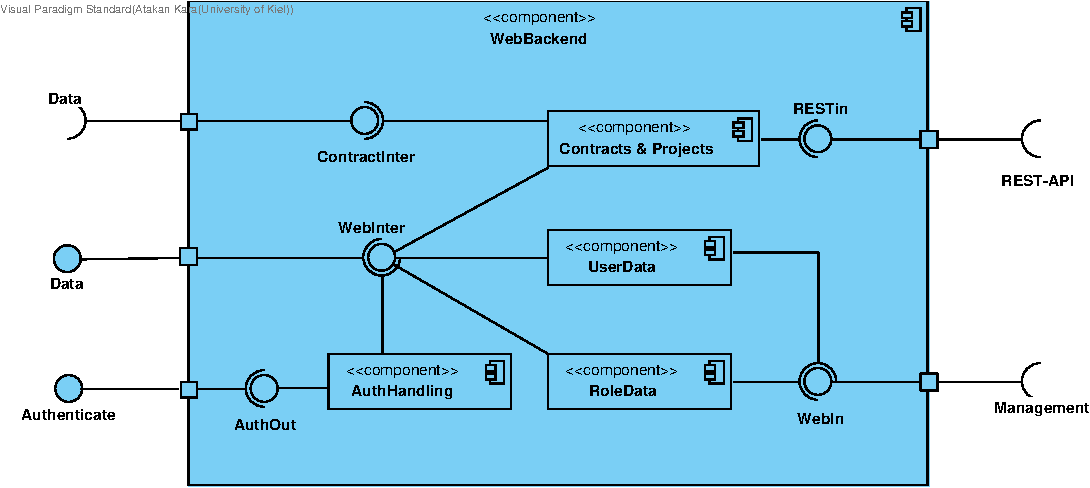
\includegraphics[width=16cm]{img/diagrams/cp_backend.pdf}	
	\caption{Komponentendiagramm - Backend}
	\label{fig:komponentendiagramm-backend}
\end{figure}

\clearpage

\begin{longtable}[h]{p{4cm} p{10.0cm}}
	\caption{Tabelle - Komponentendiagramm-Backend}
	\centering
	\label{tab:table_comp_backend}
	\endlastfoot
	\multicolumn{2}{r}{{Weitergeführt auf der folgenden Seite}} \\
	\endfoot
	\endhead
	\rowcolor[HTML]{C0C0C0} 
	\textbf{Komponente} & \textbf{Beschreibung} \\ 
	
	Authenticate & Gibt die Daten nach dem Authentifizierungsvorgang zurück. \\
	
	\rowcolor[HTML]{E7E7E7} 
	AuthHandling & Verwaltet den Authentifizierungsvorgang.  \\
	
	Contracts {\&} Projects & Speichert die Vertrags- und Projektdaten aus der \textbf{REST-API}. \\
	
	\rowcolor[HTML]{E7E7E7} 
	Data & Das eingehende Interface empfängt die Anfragen des \textbf{WebServer}s für den Erhalt und die Veränderung bestimmter Vertrags- und Projektdaten. Das ausgehende Interface gibt, falls passende Berechtigungen bestehen, die abgefragten Daten, eine Bestätigung oder eine Fehlermeldung aus.  \\
	
	Management & Nimmt Daten vom \textbf{OrgAdmin} oder \textbf{SysAdmin} entgegen und übergibt diese über das Interface \textbf{WebIn} intern der \textbf{RoleData} und \textbf{UserDate}. \\
	
	\rowcolor[HTML]{E7E7E7} 
	REST-API & Fragt die Daten von der \textbf{REST-API} ab und übergibt diese über das Interface \textbf{RESTin} der Komponente \textbf{Contracts {\&} Projects}. \\
	
	RoleData & Speichert die vom \textbf{OrgAdmin} erstellten Rollen und deren Berechtigungen ab. \\
	
	\rowcolor[HTML]{E7E7E7} 
	UserData & Speichert Nutzerdaten, wie etwa Name, Passwort und assoziierte Rolle.
\end{longtable}

\clearpage

\section{Web}

\begin{figure}[H]
	\centering
	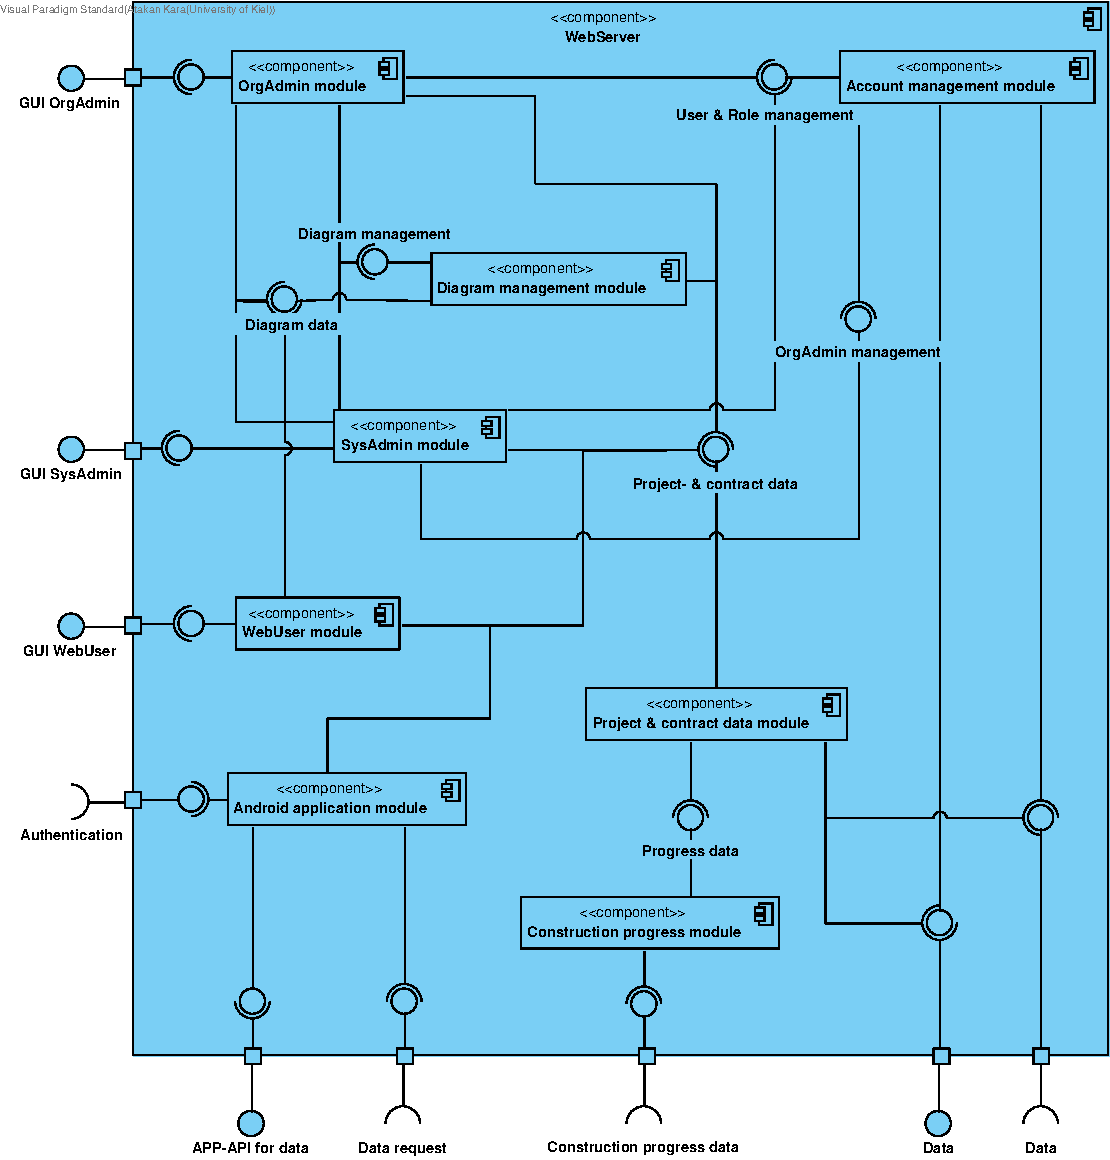
\includegraphics[width=16cm]{img/diagrams/Component-WebServer.pdf}	
	\caption{Komponentendiagramm - WebServer}
	\label{fig:komponentendiagramm-webserver}
\end{figure}

\clearpage

\begin{longtable}[h]{p{4cm} p{10.0cm}}
	\caption{Tabelle - Komponentendiagramm-WebServer}
	\centering
	\label{tab:table_comp_webserver}
	\endlastfoot
	\multicolumn{2}{r}{{Weitergeführt auf der folgenden Seite}} \\
	\endfoot
	\endhead
	\rowcolor[HTML]{C0C0C0} 
	\textbf{Komponente} & \textbf{Beschreibung} \\
	
	Account management module & Anzeige und graphische Verwaltung von \textbf{OrgAdmin}s, \textbf{WebUser} und deren Rollen. \\
	
	\rowcolor[HTML]{E7E7E7} 
	Android application module & Verwaltung der \textbf{App}. Leitet Authentifizierungs- und Datenanfragen weiter. \\
	
	APP-API for data & Schnittstelle zur Datenübermittlung zur \textbf{App}. \\
	
	\rowcolor[HTML]{E7E7E7} 
	Authentication & Schnittstelle zur Weiterleitung der Authentifizierungsanfrage des \textbf{AppUser}s zum \textbf{Backend}. \\
	
	Construction progress module & Übermittlung von Baufortschrittsdaten. \\
	
	\rowcolor[HTML]{E7E7E7} 
	Construction progress data & Eingang der Baufortschrittsdaten der App, wie z.B. Fotos und deren Beschreibungen. \\
	
	Data & Ein- und Ausgang von Projekt-, Vertrags-, und Kontodaten zum und vom \textbf{Backend}. \\
	
	\rowcolor[HTML]{E7E7E7} 
	Data request & Erhalt der Anfragen zur Datenübermittlung von der \textbf{App}. \\
	
	Diagram management module & Verwaltung und Anzeige von Diagrammen. \\
	
	\rowcolor[HTML]{E7E7E7} 
	Project {\&} contract data module & Verwaltung und Weiterleitung von Projekt- und Vertragsdaten. \\
	
	GUI OrgAdmin & Eingehende Daten und graphische Nutzeroberfläche des \textbf{OrgAdmin}s. Dieser muss eingeloggt sein. \\
	
	\rowcolor[HTML]{E7E7E7} 
	GUI SysAdmin & Eingehende Daten und graphische Nutzeroberfläche des \textbf{SysAdmin}s. Dieser muss eingeloggt sein. \\
	
	GUI WebUser & Eingehende Daten und graphische Nutzeroberfläche des \textbf{WebUser}s. Dieser muss eingeloggt sein. \\
	
	\rowcolor[HTML]{E7E7E7} 
	OrgAdmin module & Vereinigt die Interaktionsmöglichkeiten des \textbf{OrgAdmin}s in einem zentralen Modul. \\
	
	SysAdmin module & Vereinigt die Interaktionsmöglichkeiten des \textbf{SysAdmin}s in einem zentralen Modul. \\
	
	\rowcolor[HTML]{E7E7E7} 
	WebUser module & Vereinigt die Interaktionsmöglichkeiten des \textbf{AppUser}s in einem zentralen Modul.
\end{longtable}

\clearpage

\section{App}

\begin{figure}[H]
	\centering
	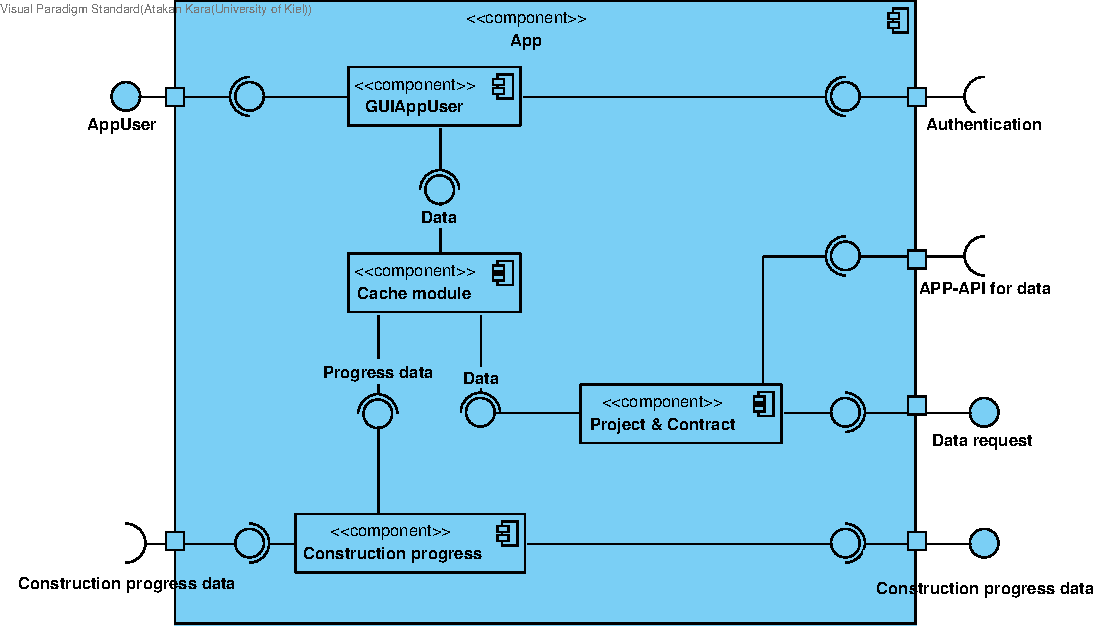
\includegraphics[width=16cm]{img/diagrams/Component-App.pdf}
	\caption{Komponentendiagramm - App}
	\label{fig:komponentendiagramm-app}
\end{figure}


\begin{longtable}[h]{p{4cm} p{10.0cm}}
	\caption{Tabelle - Komponentendiagramm-App}
	\centering
	\label{tab:table_comp_app}
	\endlastfoot
	\multicolumn{2}{r}{{Weitergeführt auf der folgenden Seite}} \\
	\endfoot
	\endhead
	\rowcolor[HTML]{C0C0C0} 
	\textbf{Komponente} & \textbf{Beschreibung} \\ 
	
	AppUser & Einsicht der Daten für den Nutzer der Applikation. \\
	
	\rowcolor[HTML]{E7E7E7} 
	APP-API for data & Erhalt von Projekt- und Vertragsdaten vom \textbf{WebServer}. \\
	
	Authentication & Übermittelt notwendige Daten zum \textbf{WebServer} zur Authentifizierung des \textbf{AppUser}s. \\
	
	\rowcolor[HTML]{E7E7E7} 
	Cache module & Dient der Zwischenspeicherung der Projekt- und Vertragsdaten sowie des Baufortschritts. \\
	
	Construction progress & Verwaltet den Baufortschritt. \\
	
	\rowcolor[HTML]{E7E7E7} 
	Construction progress data & Das eingehende Interface erhält Daten zum Baufortschritt, wie z.B. Fotos und deren Beschreibungen. Diese fügt der \textbf{AppUser} hinzu. Das ausgehende Interface hingegen übermittelt diese an den \textbf{WebServer}. \\
	
	Data request & Schnittstelle zur Anfrageübermittlung zum \textbf{WebServer}. \\
	
	\rowcolor[HTML]{E7E7E7} 
	GUIAppUser & Modul zur Darstellung der graphischen Nutzeroberfläche der \textbf{App}. \\
	
	Project {\&} Contract & Verwaltet die Projekt- und Vertragsdaten.
\end{longtable}

\clearpage